\section{Related Work}

As we do not propose any kind of new algorithm, we will make use of existing solutions for both
the computation of the colour corrected image, and the actual classification of the images.

\subsection{Color Constancy}

\begin{figure}
    \centering
    \begin{tabular}{cccc}
    \bmvaHangBox{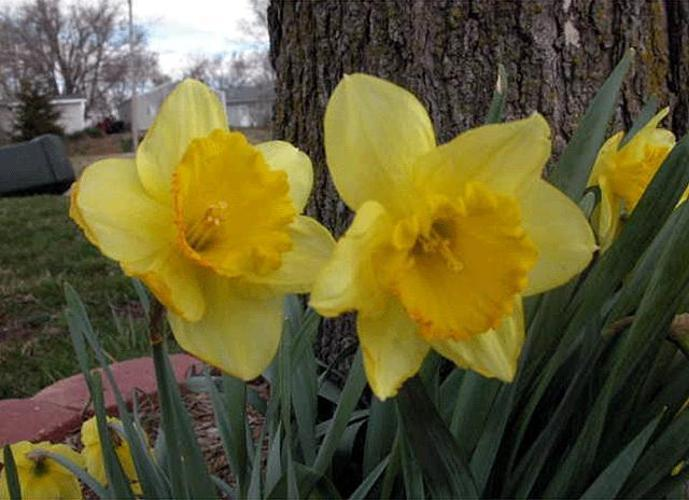
\includegraphics[width=0.2\textwidth]{cc_demo/flower001_base.png}}&
    \bmvaHangBox{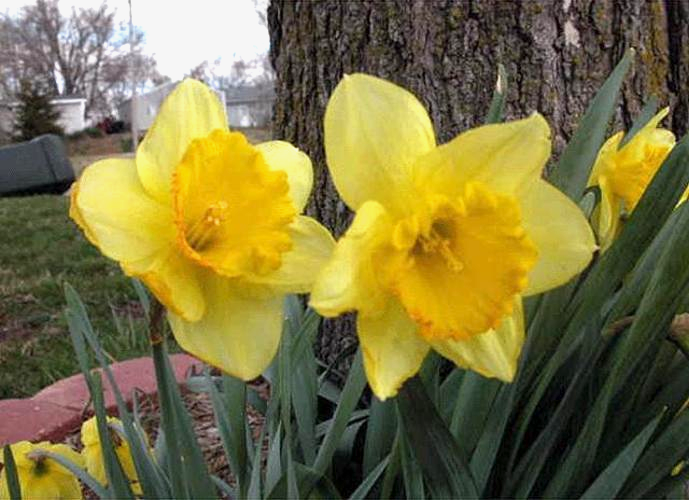
\includegraphics[width=0.2\textwidth]{cc_demo/flower001_whitePatch.png}}&
    \bmvaHangBox{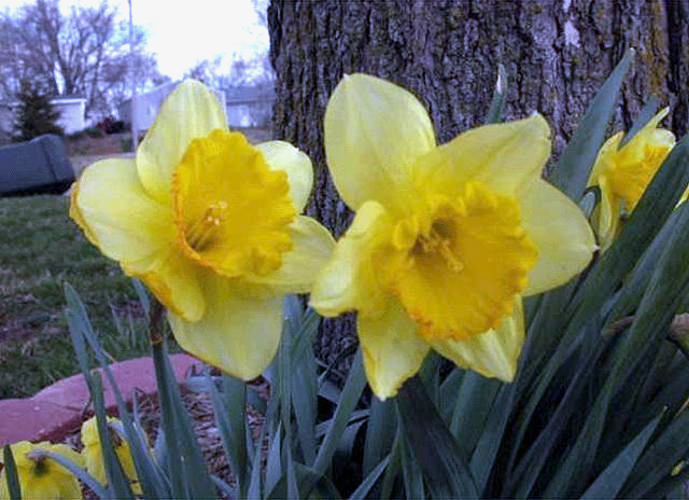
\includegraphics[width=0.2\textwidth]{cc_demo/flower001_greyWorld.png}}&
    \bmvaHangBox{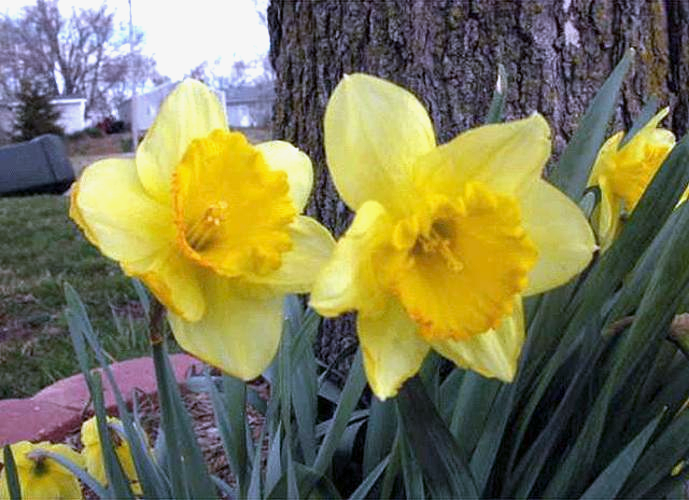
\includegraphics[width=0.2\textwidth]{cc_demo/flower001_grayEdge.png}}\\
    (a)&(b)&(c)&(d)\\
    \bmvaHangBox{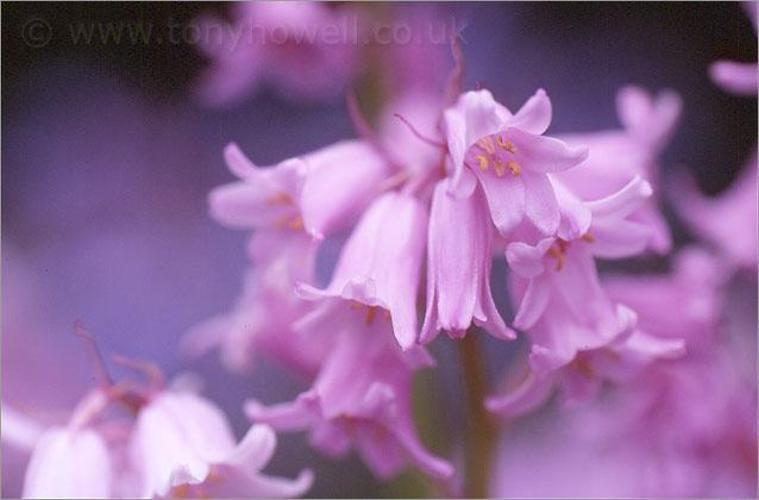
\includegraphics[width=0.2\textwidth]{cc_demo/flower268_base.png}}&
    \bmvaHangBox{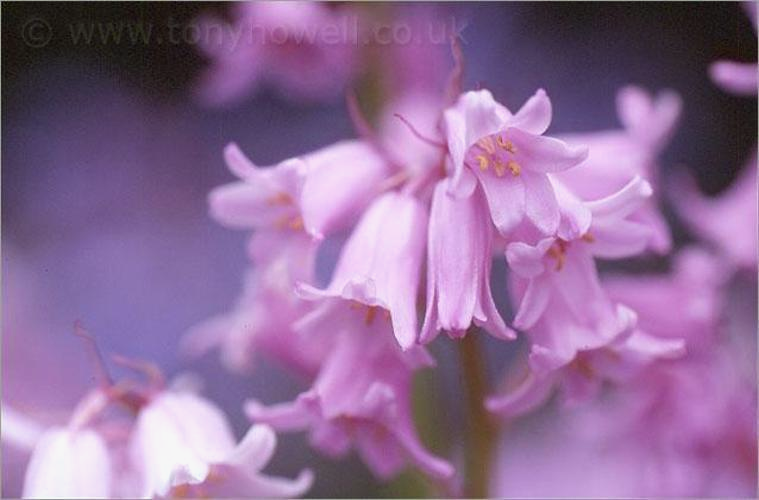
\includegraphics[width=0.2\textwidth]{cc_demo/flower268_whitePatch.png}}&
    \bmvaHangBox{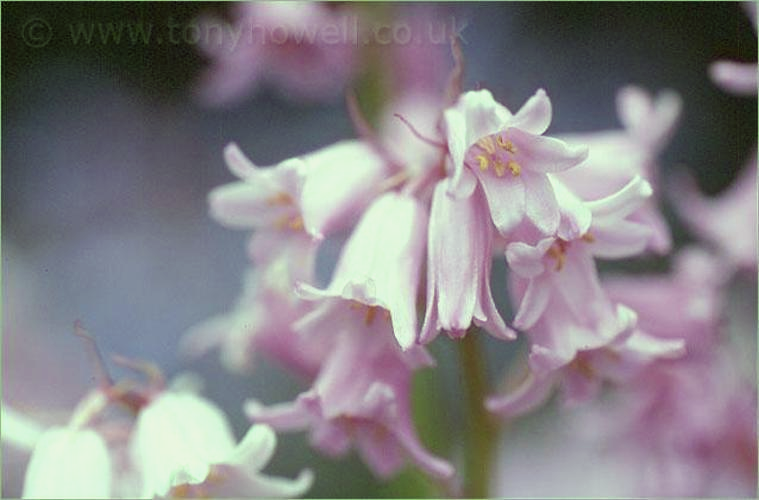
\includegraphics[width=0.2\textwidth]{cc_demo/flower268_greyWorld.png}}&
    \bmvaHangBox{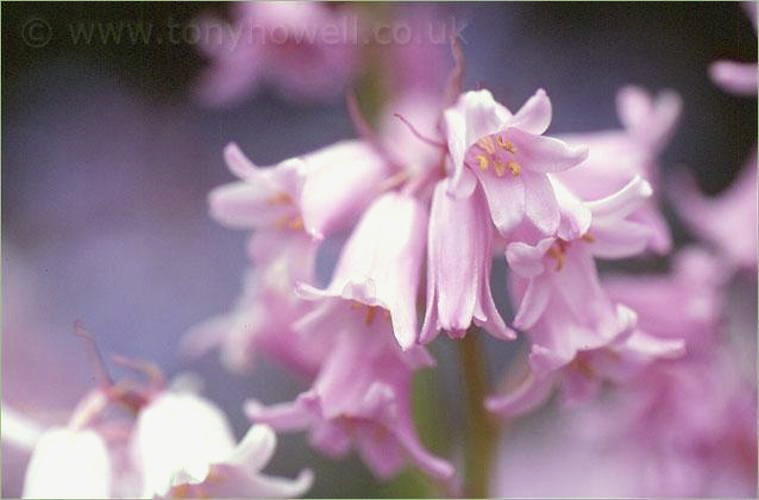
\includegraphics[width=0.2\textwidth]{cc_demo/flower268_grayEdge.png}}\\
    (e)&(f)&(g)&(h)
    \end{tabular}
    \caption{A comparison of color constancy algorithms: (a) and (e): Original image.
        (b) and (f): White Patch. (c) and (g): Grey-World. (d) and (h): Grey-Edge.}
    \label{fig:cc_comparison}
\end{figure}

In order to have a wider spread of examined methods, we both make use of state-of-the art 
learning based methods like CLCC \cite{Lo_2021_CVPR}, as well as classical simpler methods 
like White-Patch, Grey-World \cite{EbnerConstancy} and Grey-Edge \cite{van2005color}.
A comparison of these can be found in \ref{fig:cc_comparison}.

To evaluate our results we can make use of the publicly available Oxford 17 \cite{Nilsback06} 
and Oxford 104 \cite{Nilsback08} class datasets.

